\documentclass[a4paper, 12pt]{article}

\usepackage{cmap}
\usepackage{mathtext} 
\usepackage[T2A]{fontenc}
\usepackage[utf8]{inputenc}
\usepackage[english,russian]{babel}	

\usepackage{amsfonts,amssymb,amsthm,mathtools}
\usepackage{amsmath}
\usepackage{icomma} 

\usepackage{graphicx} 
\graphicspath{{Picturies/}}
\usepackage{wrapfig}

\usepackage{array,tabularx,tabulary,booktabs}
\usepackage{longtable}
\usepackage{multirow}

\usepackage{caption}
\captionsetup{labelsep=period}

\renewcommand{\phi}{\varphi}
\newcommand{\eps}{\varepsilon}
\renewcommand{\AA}{\ensuremath{\mathring{A}}}
\newcommand{\parag}[1]{\paragraph*{#1:}}

\newcounter{Points}
\setcounter{Points}{1}
\newcommand{\point}{\arabic{Points}. \addtocounter{Points}{1}}

\author{Вязовцев Андрей, Б01-009}
\date{09.10.22}
\title{Лабораторная работа 5.8.1. }

\begin {document}

\maketitle

\parag {Цель работы} при помощи модели абсолютно чёрного тела (АЧТ) проводятся измерения температуры, исследуется излучение накалённых тел, определяются постоянные Планка и Стефана-Больцмана. 

\parag {В работе используются} оптический пирометр с исчезающей нитью и термопарой, накалённые тела с различной испускательной способностью.

\parag {Теоретическая справка} ~\\

Для измерения температуры тел, удалённых от наблюдателя, применяют методы оптических пирометрии, основанные на использовании зависимости испускательной способности исследуемого тела от температуры. Различают три температуры, функционально связанные с истинной термодинамической температурой и излучательной способностью тела: радиационную $T_{рад}$, цветовую $T_{цв}$ и яркостную $T_{ярк}$.

Радиационная (энергетическая) температура --- температура АЧТ, при которой его интегральная испускательная способность одинакова с интегральной испускательной способностью исследуемого тела.

Цветовая температура --- температура АЧТ, при которой отношение их спектральных испускательных способностей для двух заданных длин волн одинаково.

Яркостная температура --- температура АЧТ, при которой его спектральная испускательная способность равна спектральной испукательной способности исследуемого тела при той же длине волны. Именно эту температуру мы и будем измерять. Для вольфрама функциональная зависимость термодинамической температуры от яркостной представлена на рис. \ref{th:1}.

\begin{figure}[!h]
    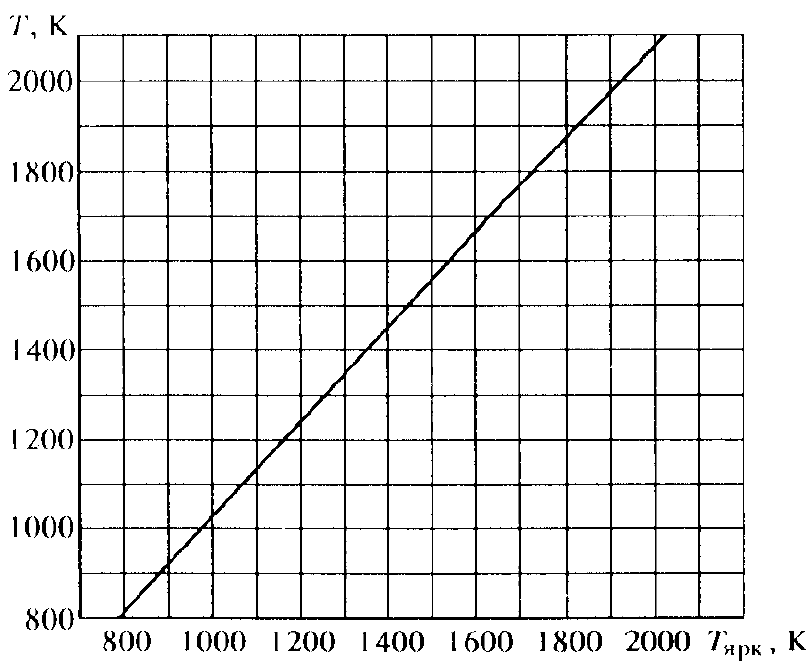
\includegraphics[scale = 0.4]{Brightness}
    \centering
    \caption{$T = f(T_{ярк})$ для вольфрама}
    \label{th:1}
\end{figure}

Закон Киргофа для излучения любого тела:

\begin{equation}
    r_{\lambda} = a_{\lambda} r_{\lambda}^{АЧТ}
\end{equation}

Для абсолютно серого тела (АСТ):

\begin{equation}
    a_{\lambda} \equiv a = const
\end{equation}

Если бы нить излучала как АЧТ, то баланс потребляемой и излучаемой энергии определялся бы соотношением:

\begin{equation}
    W = \sigma S (T^4 - T_0^4)
\end{equation}

где $W$ --- потребляемой нитью электрическая мощность, $S$ --- площадь излучаемой поверхности нити, $T$ --- температура нити, $T_0$ --- температура окружающей среды, $\sigma = 5.67 \cdot 10^{-12} ~ \dfrac{Вт}{см^2 \cdot К^4}$ --- постоянная Стефана-Больцмана.

Если считать нить серым телом и его излучение ослаблено на $\eps_T$ по сравнению с АЧТ, то:

\begin{equation} \label{eq:s-b}
    W = \eps_T S \sigma T^4
\end{equation}

Коэффициент $\eps_T$ зависит от температуры следующим образом для вольфрама:

\begin{table}[!h]
    \centering
    \begin{tabular}{|c|c|c|c|c|}
        \hline
        $T$, К  &   1700 &  1800 &  1900 &  2000 \\ \hline
        $\eps_T$ & 0.209 & 0.223 & 0.236 & 0.249 \\ \hline
    \end{tabular}
    \caption {$\eps_T (T)$ для вольфрама}
    \label{tab:epsT}
\end{table}

При выполнении работы также потребуется вычислить постоянную планка $h$ с помощью постоянной Стефана-Больцмана $\sigma$. Приведём необходимую формулу ниже:

\begin{equation} \label{eq:h-sigma}
    h = \sqrt[3]{\frac{2 \pi^5 k_Б^4}{15 c^2 \sigma}}
\end{equation}

\parag {Экспериментальная установка} ~

На рис. \ref{pic:work} изображена экспериментальная установка. Она состоит из оптического пирометра 9, модели АЧТ, трёх образцов (18, 19, 20), блока питания (1) и цифровых вольтметров В7-22А и В7-38.

\begin{enumerate}
    \item Блок питания
    \item Тумблер включения питания пирометра и образцов
    \item Тумблер нагрева нити пирометра <<Быстро>> --- вверх, <<Медленно>> --- вниз
    \item Кнопка <<Нагрев нити>>
    \item Кнопка <<Охлаждение нити>>
    \item Тумблер переключения образцов
    \item Регулятор мощности нагрева образцов
    \item Окуляр пирометра
    \item Корпус пирометра
    \item Объектив пирометра
    \item Переключение диапазонов: $700-1200 ~^\circ C$ --- вниз, $1200-2000 ~^\circ C$ --- вверх
    \item Ручка перемещения красного светофильтра
    \item Регулировочный винт
    \item Вольтметр (напряжение на лампе накаливания)
    \item Амперметр (ток через образцы)
    \item Вольтметр в цепи термопары
    \item Модель АЧТ
    \item Трубка с кольцами из материалов с разной излучательной способностью
    \item Лампа накаливания
    \item Неоновая лампочка
\end{enumerate}

\begin{figure}[!h]
    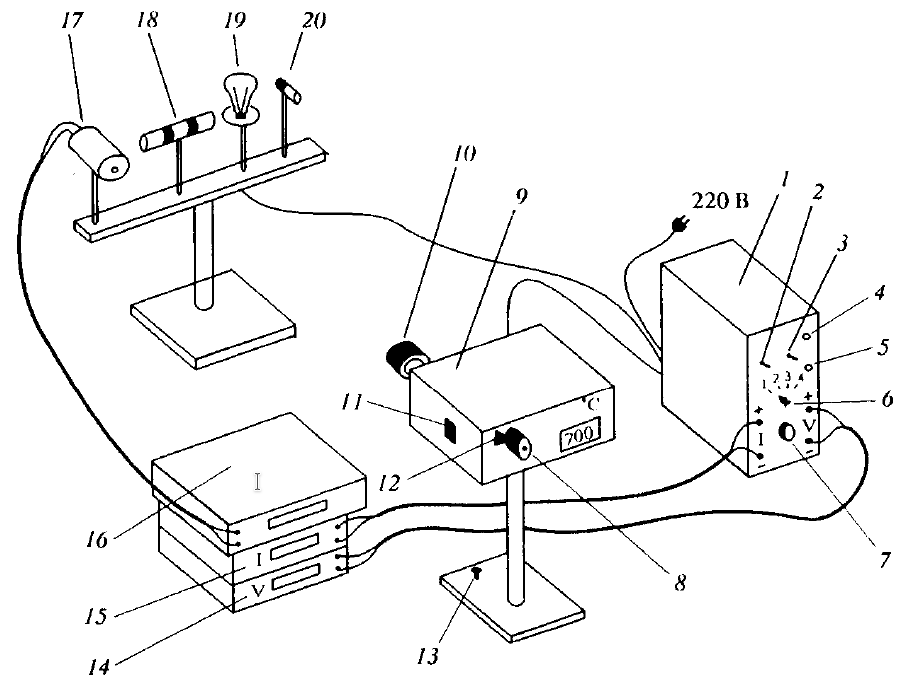
\includegraphics[scale = 0.4]{Workplace}
    \centering
    \caption{Схема экспериментальной установки.}
    \label{pic:work}
\end{figure}

\parag {Ход работы} ~\\

\parag {I. Изучение работы оптического пирометра.} ~\\

\point Включим модель АЧТ, дадим ей прогреться (приблизительно до $37.5$ мВ на термопаре). Далее включиим пирометр и измерим температуру (температуры тела и нити считаются равными, когда нить сливается с ним). Также укажем ожидаемую температуру (используя постоянную термопары $41$ мкВ).

\begin{table}[!h]
    \centering
    \begin{tabular}{|c|c|c|c|c|}
        \hline
        направление & вверх & вверх & вниз & вниз \\ \hline
        $U$, мВ & 37.97 & 37.91 & 38.04 & 37.92 \\ \hline
        $T_{ярк}$  & 926 & 937 & 934 & 938 \\ \hline
        $T_{терм}$ & 926 & 925 & 928 & 925 \\ \hline
    \end{tabular}
    \caption {Измерения на АЧТ}
    \label{tab:1}
\end{table}

Из таблицы видно, что температуры отличаются в пределах $3\%$, т.~е. пирометр настроен верно. 

\newpage

\parag {II. Измерение яркостной температуры накалённых тел.} ~\\

\point Посмотрим, как различные тела при одной и той же температуре имеют яркостную температуру. Для этого измерим температуру колец. Результаты см. в таблице \ref{tab:2}.

\begin{table}[!h]
    \centering
    \begin{tabular}{|c|c|c|c|}
        \hline
        объект & левое кольцо & керамика & правое кольцо \\ \hline
        $T, ~^\circ C$ & 800 & 846 & 784 \\ \hline
    \end{tabular}
    \caption {Кольца}
    \label{tab:2}
\end{table}

\newpage

\parag {III. Проверка закона Стефана-Больцмана.} ~\\

\point Теперь измерим напряжение и силу тока через лампочу с нитью накаливания прощадью $S = 0.36 ~ см^2$, изменяя её яркостную температуру от $900$ до $1900 ~^\circ C$. Результаты представлены в таблице \ref{tab:3}.

\begin{table}[!h]
    \centering
    \begin{tabular}{|c|c|c|c|c|c|c|}
        \hline
        $T_{ярк}, ~^\circ C$ & 900 & 1000 & 1100 & 1200 & 1300 & 1400 \\ \hline
        $U$, В & 1.710 & 1.973 & 2.449 & 2.942 & 3.214 & 3.891 \\ \hline
        $I$, А & 0.485 & 0.511 & 0.558 & 0.603 & 0.627 & 0.684 \\ \hline
    \end{tabular}
    \\~\\~
    \begin{tabular}{|c|c|c|c|c|c|}
        \hline
        $T_{ярк}, ~^\circ C$ & 1500 & 1600 & 1700 & 1800 & 1900 \\ \hline
        $U$, В & 4.660 & 5.287 & 6.243 & 7.245 & 7.797 \\ \hline
        $I$, А & 0.745 & 0.793 & 0.861 & 0.929 & 0.964 \\ \hline
    \end{tabular}
    \caption {Лампа}
    \label{tab:3}
\end{table}

\point Теперь определим с помощью этих данных выделяемую на лампе мощность и термодинамическую температуру (с помощью графика \ref{th:1}).

\begin{table}[!h]
    \centering
    \begin{tabular}{|c|c|c|c|c|c|c|}
        \hline
        $T_{ярк}, ~^\circ C$ &  900 & 1000 & 1100 & 1200 & 1300 & 1400 \\ \hline
        $T_{терм}$, К        & 1210 & 1320 & 1430 & 1530 & 1640 & 1740 \\ \hline
        $W$, Вт              & 0.83 & 1.01 & 1.37 & 1.77 & 2.02 & 2.66 \\ \hline
    \end{tabular}
    \\~\\~
    \begin{tabular}{|c|c|c|c|c|c|}
        \hline
        $T_{ярк}, ~^\circ C$  & 1500 & 1600 & 1700 & 1800 & 1900 \\ \hline
        $T_{терм}$, К         & 1850 & 1960 & 2060 & 2170 & 2270 \\ \hline
        $W$, Вт               & 3.47 & 4.19 & 5.38 & 6.73 & 7.52 \\ \hline
    \end{tabular}
    \caption {Ещё лампа}
    \label{tab:4}
\end{table}

\point Построим графики $W = f(T)$ (см. рис. \ref{pic:W}) и $\ln W = f(\ln T) = \ln (\eps_T \sigma S) + n \ln T$ (см. рис. \ref{pic:lnW}). 

\begin{figure}[!h]
    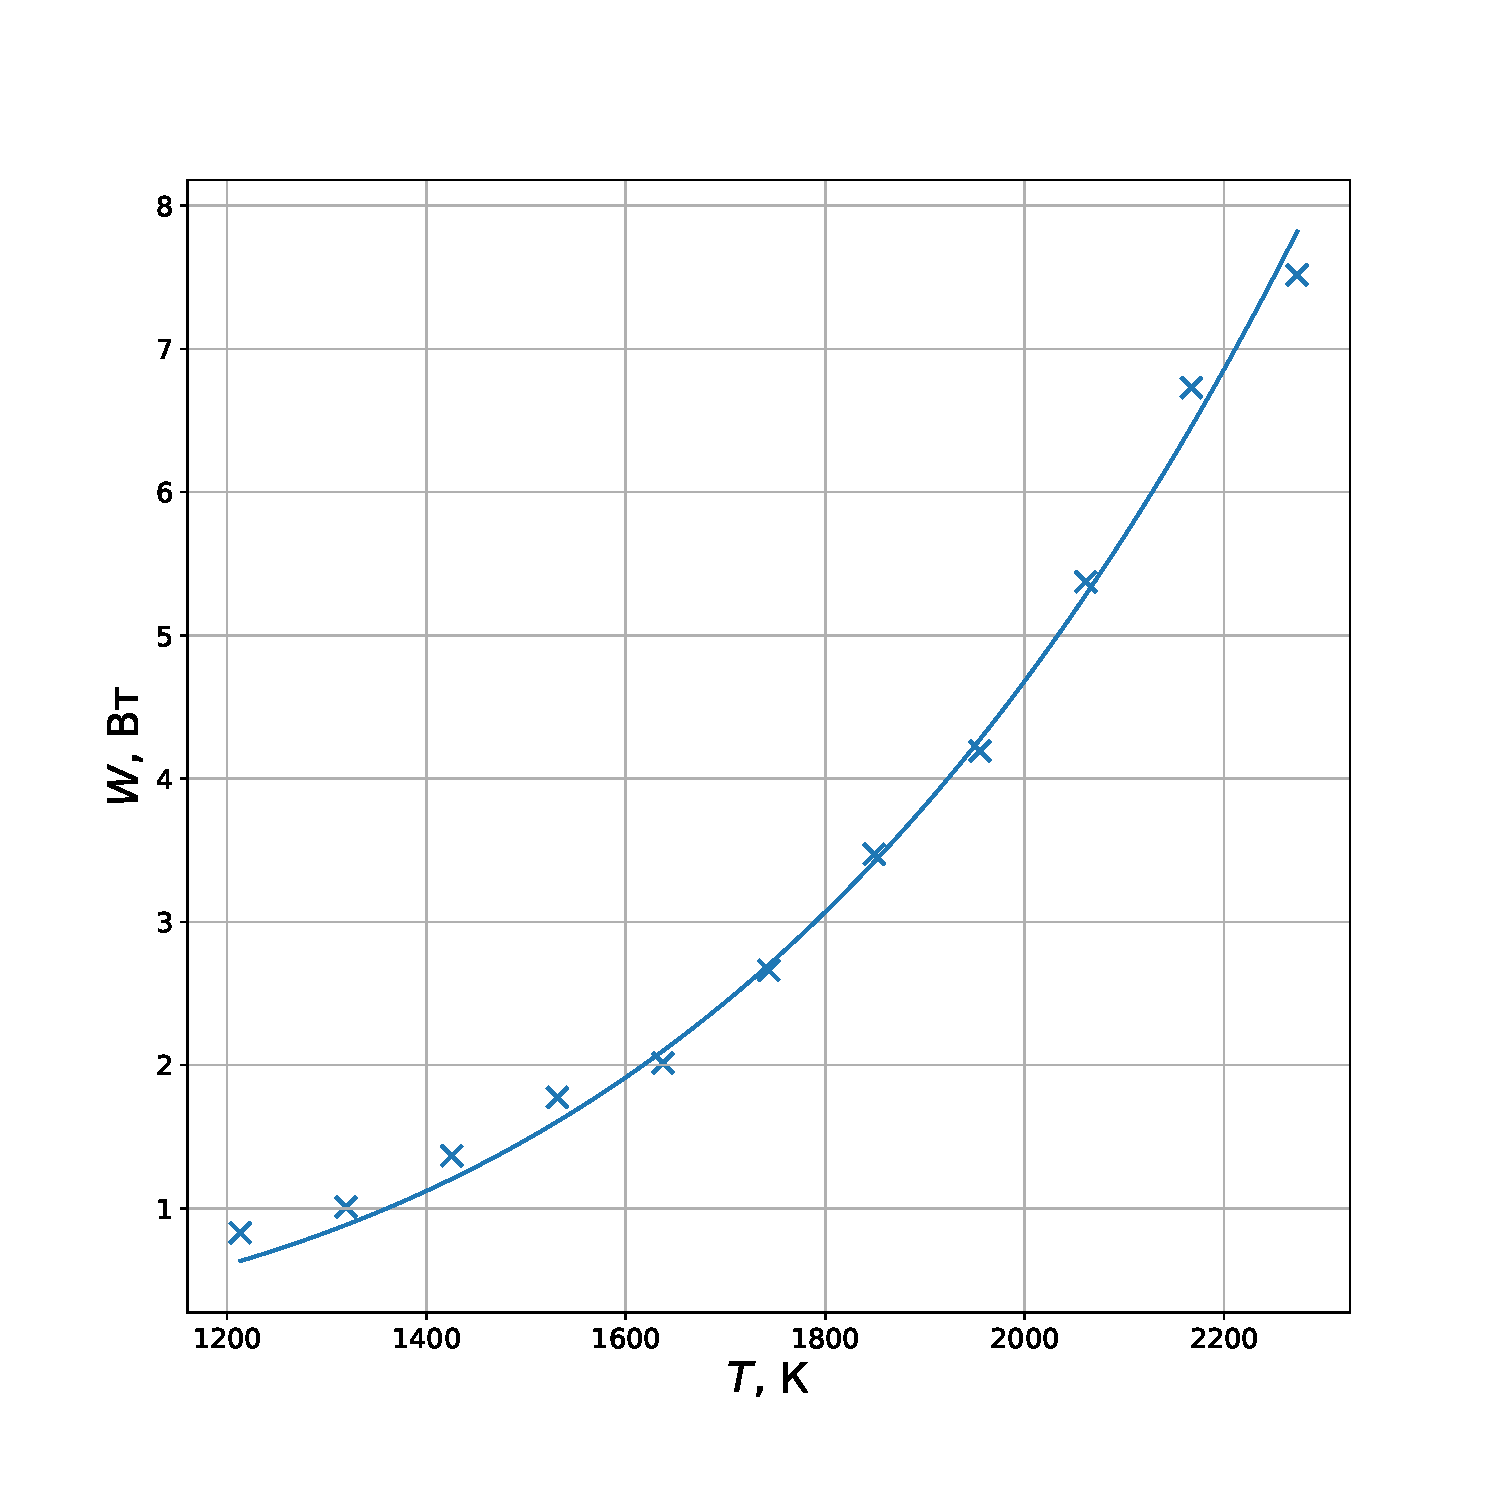
\includegraphics[scale = 0.4]{graphW}
    \centering
    \caption{График $W = f(T)$}
    \label{pic:W}
\end{figure}

\begin{figure}[!h]
    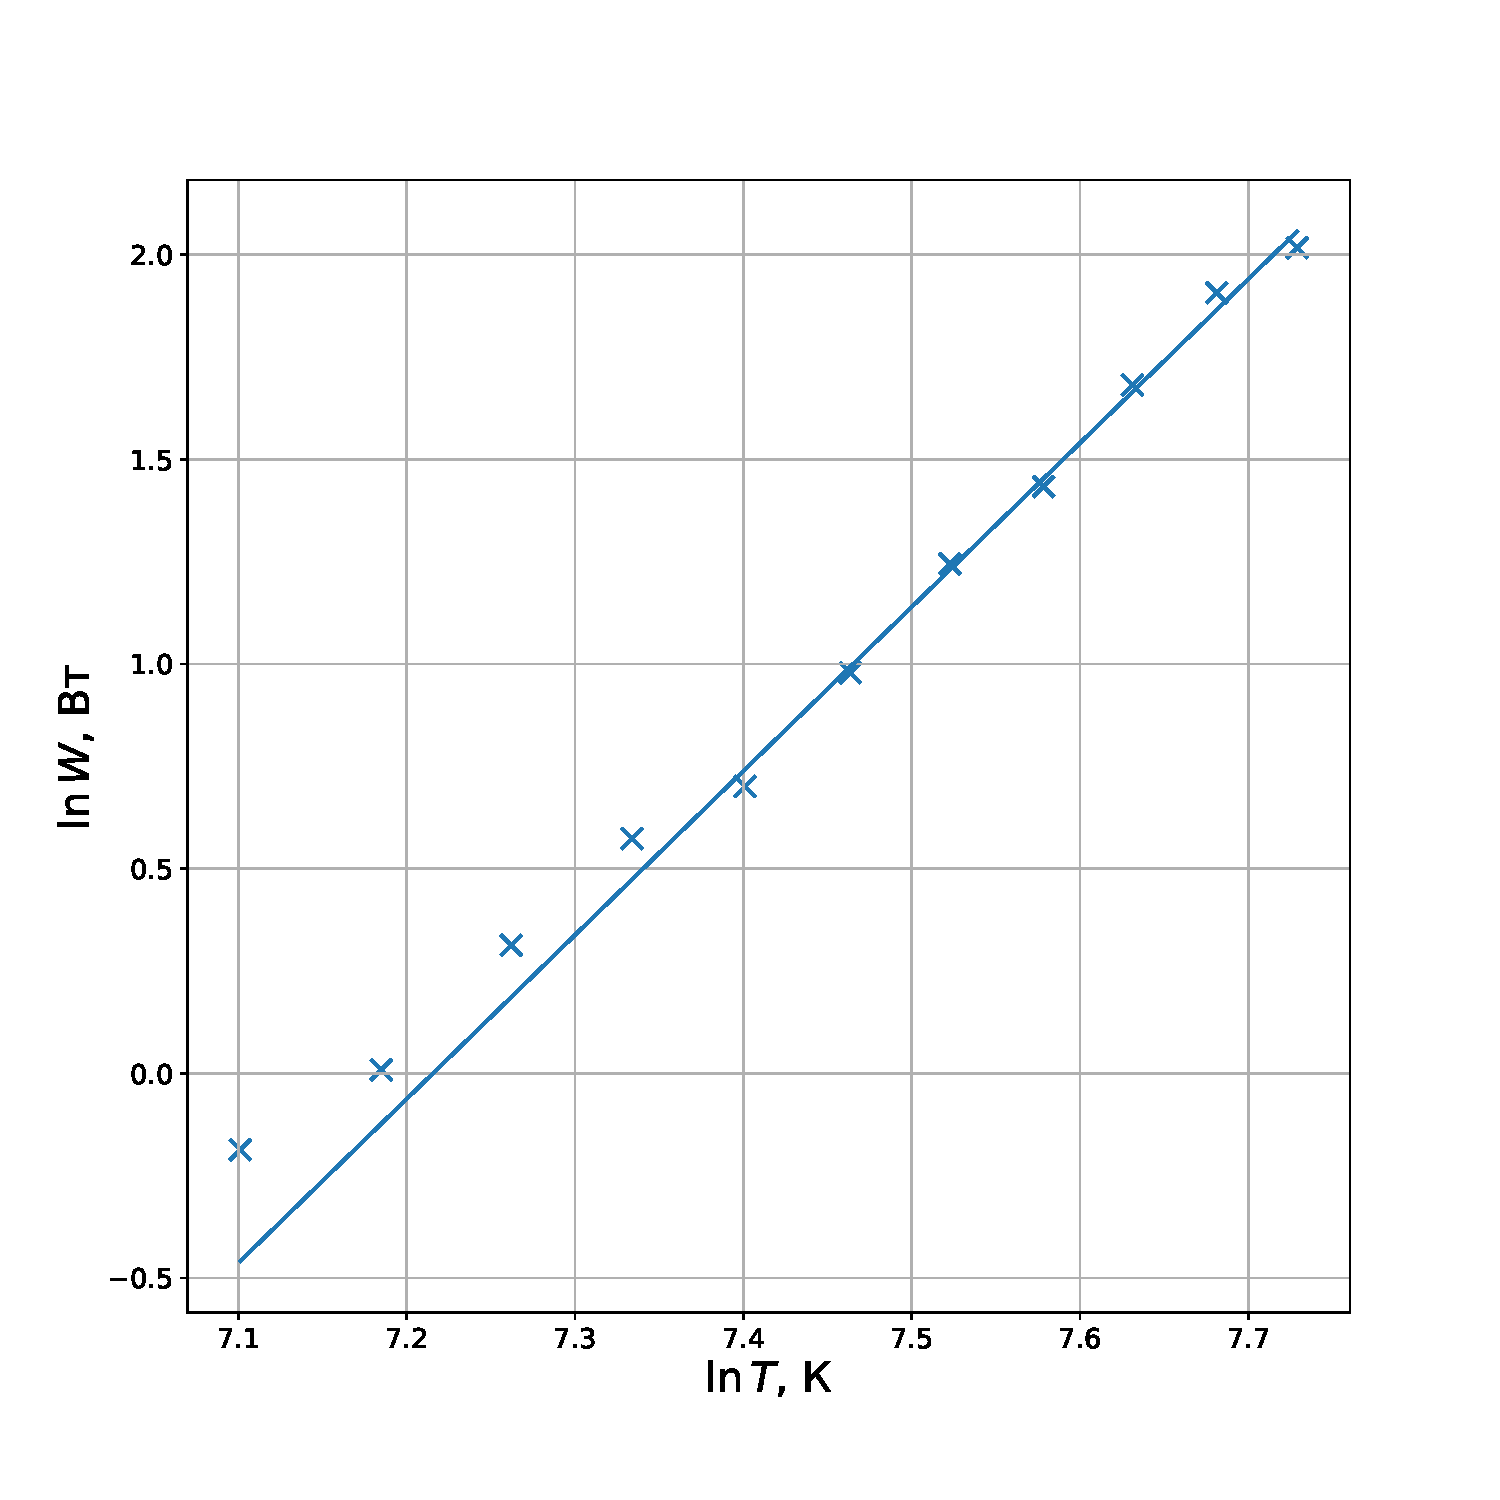
\includegraphics[scale = 0.4]{graphlnW}
    \centering
    \caption{График $\ln W = f(\ln T)$}
    \label{pic:lnW}
\end{figure}

\point Из графика с помощью МНК получаем:

\begin{align*}
    n &= 4.01 \pm 0.12 \\
    \ln (\eps_T \sigma S) &= -26.91 \pm 0.01
\end{align*}

Стоит отметить, что график строился только по тем точкам, у которых $T > 1700$ К. Это сделано из-за того, что при меньших температурах существует зависимость $S(T)$, которую невозможно учесть. Начиная же с таких температур нить накаляется полностью, т.~е. $S = 0.36~см^2 = const$. Но при этом необходимо учесть, что $\eps_T$ тоже зависит от температуры. Для этого была использована таблица \ref{tab:epsT}.

Также заметим, что теоретическое значение $n = 4$ (см. \eqref{eq:s-b}). Полученное экспериментальное значение сходится с теоретическим. Звучит нереалистично.

\point Для каждого значения $T > 1700$ К найдём постоянную Стефана-Больцмана по формуле \ref{eq:s-b}. Результаты представлены в таблице \ref{tab:sigma}.

\begin{table}[!h]
    \centering
    \begin{tabular}{|c|c|c|c|c|c|c|}
        \hline
        $T$, К   &   1740 &  1850 &  1960 &  2060 & 2170 & 2270 \\ \hline
        $\sigma, \dfrac{Вт}{см^2 \cdot К^4}$ & $3.76 \cdot 10^{-12}$ & $3.62 \cdot 10^{-12}$ & $3.28 \cdot 10^{-12}$ & $3.21 \cdot 10^{-12}$ & $3.11 \cdot 10^{-12}$ & $2.72 \cdot 10^{-12}$ \\ \hline
    \end{tabular}
    \caption {$\sigma (T)$}
    \label{tab:sigma}
\end{table}

Как видно, полученные значения отличаются в $1.5$-$2$ раза. Вероятно, проблема в неверно указанном $S$ на установке.

\point Теперь с помощью формулы \eqref{eq:h-sigma} найдём постоянную планка. Очевидно, что оно будет неверно, ну да и ладно. Результаты --- в табл. \ref{tab:h}.

\begin{table}[!h]
    \centering
    \begin{tabular}{|c|c|c|c|c|c|c|}
        \hline
        $T$, К   &   1740 &  1850 &  1960 &  2060 & 2170 & 2270 \\ \hline
        $h, Дж \cdot с$ & $7.60 \cdot 10^{-34}$ & $7.69 \cdot 10^{-34}$ & $7.95 \cdot 10^{-34}$ & $8.01 \cdot 10^{-34}$ & $8.10 \cdot 10^{-34}$ & $8.47 \cdot 10^{-34}$ \\ \hline
    \end{tabular}
    \caption {$h (T)$}
    \label{tab:h}
\end{table}

\newpage

\parag {IV. Измерение <<яркостной температуры>> неоновой лампочки.} ~\\

\point Теперь направим пирометр на неоновую лампочку. Находим $T_{ярк} = 830$ К. Но при этом она холодная на ощупь. Это означается, что природа свечения в ней другая.

% \parag {Обработка результатов} ~\\

% \point 

\end {document}
